% Section fragment; requires graphicx and hyperref in the main document.
% Figure paths are relative to the project root.
% Source markers retain the Markdown hyperlinks; they are not bibliography citations.
\section{数据处理和探索性分析}
\label{sec:frontmatter-data-exploration}

\subsection{数据处理}

经检查，四个附件的有效数值字段未发现缺失值、非有限值或负功率，电价均为正值，日期与时段的对应关系完整。因此，数据无需进行缺失值插补、异常值修正等额外预处理，可直接用于后续分析。

\subsection{探索性分析}

微网购电既要满足负载，又要兼顾光伏消纳和运行经济性。围绕这三者的关系，我们从日内供需、月度变化、负载周期以及预报与电价变化四个方面展开分析。

\subsubsection{日内供需匹配与储能调度空间}

考虑到光伏发电依赖日照，而居民用电遵循生活作息，两者在时间上未必一致。相关资料也指出，太阳能发电充裕的时刻并不总是用电需求最大的时刻，储能的重要作用之一正是缓解这种时间错位。\textsuperscript{\href{https://www.energy.gov/cmei/systems/solar-integration-solar-energy-and-storage-basics}{[1]}} 因此，我们将附件1的负载、光伏预测功率及电价放在同一日内尺度下比较，并以负载电量减去光伏电量定义净负荷，绘得图~\ref{fig:eda-daily-conditions}。

\begin{figure}[!htbp]
  \centering
  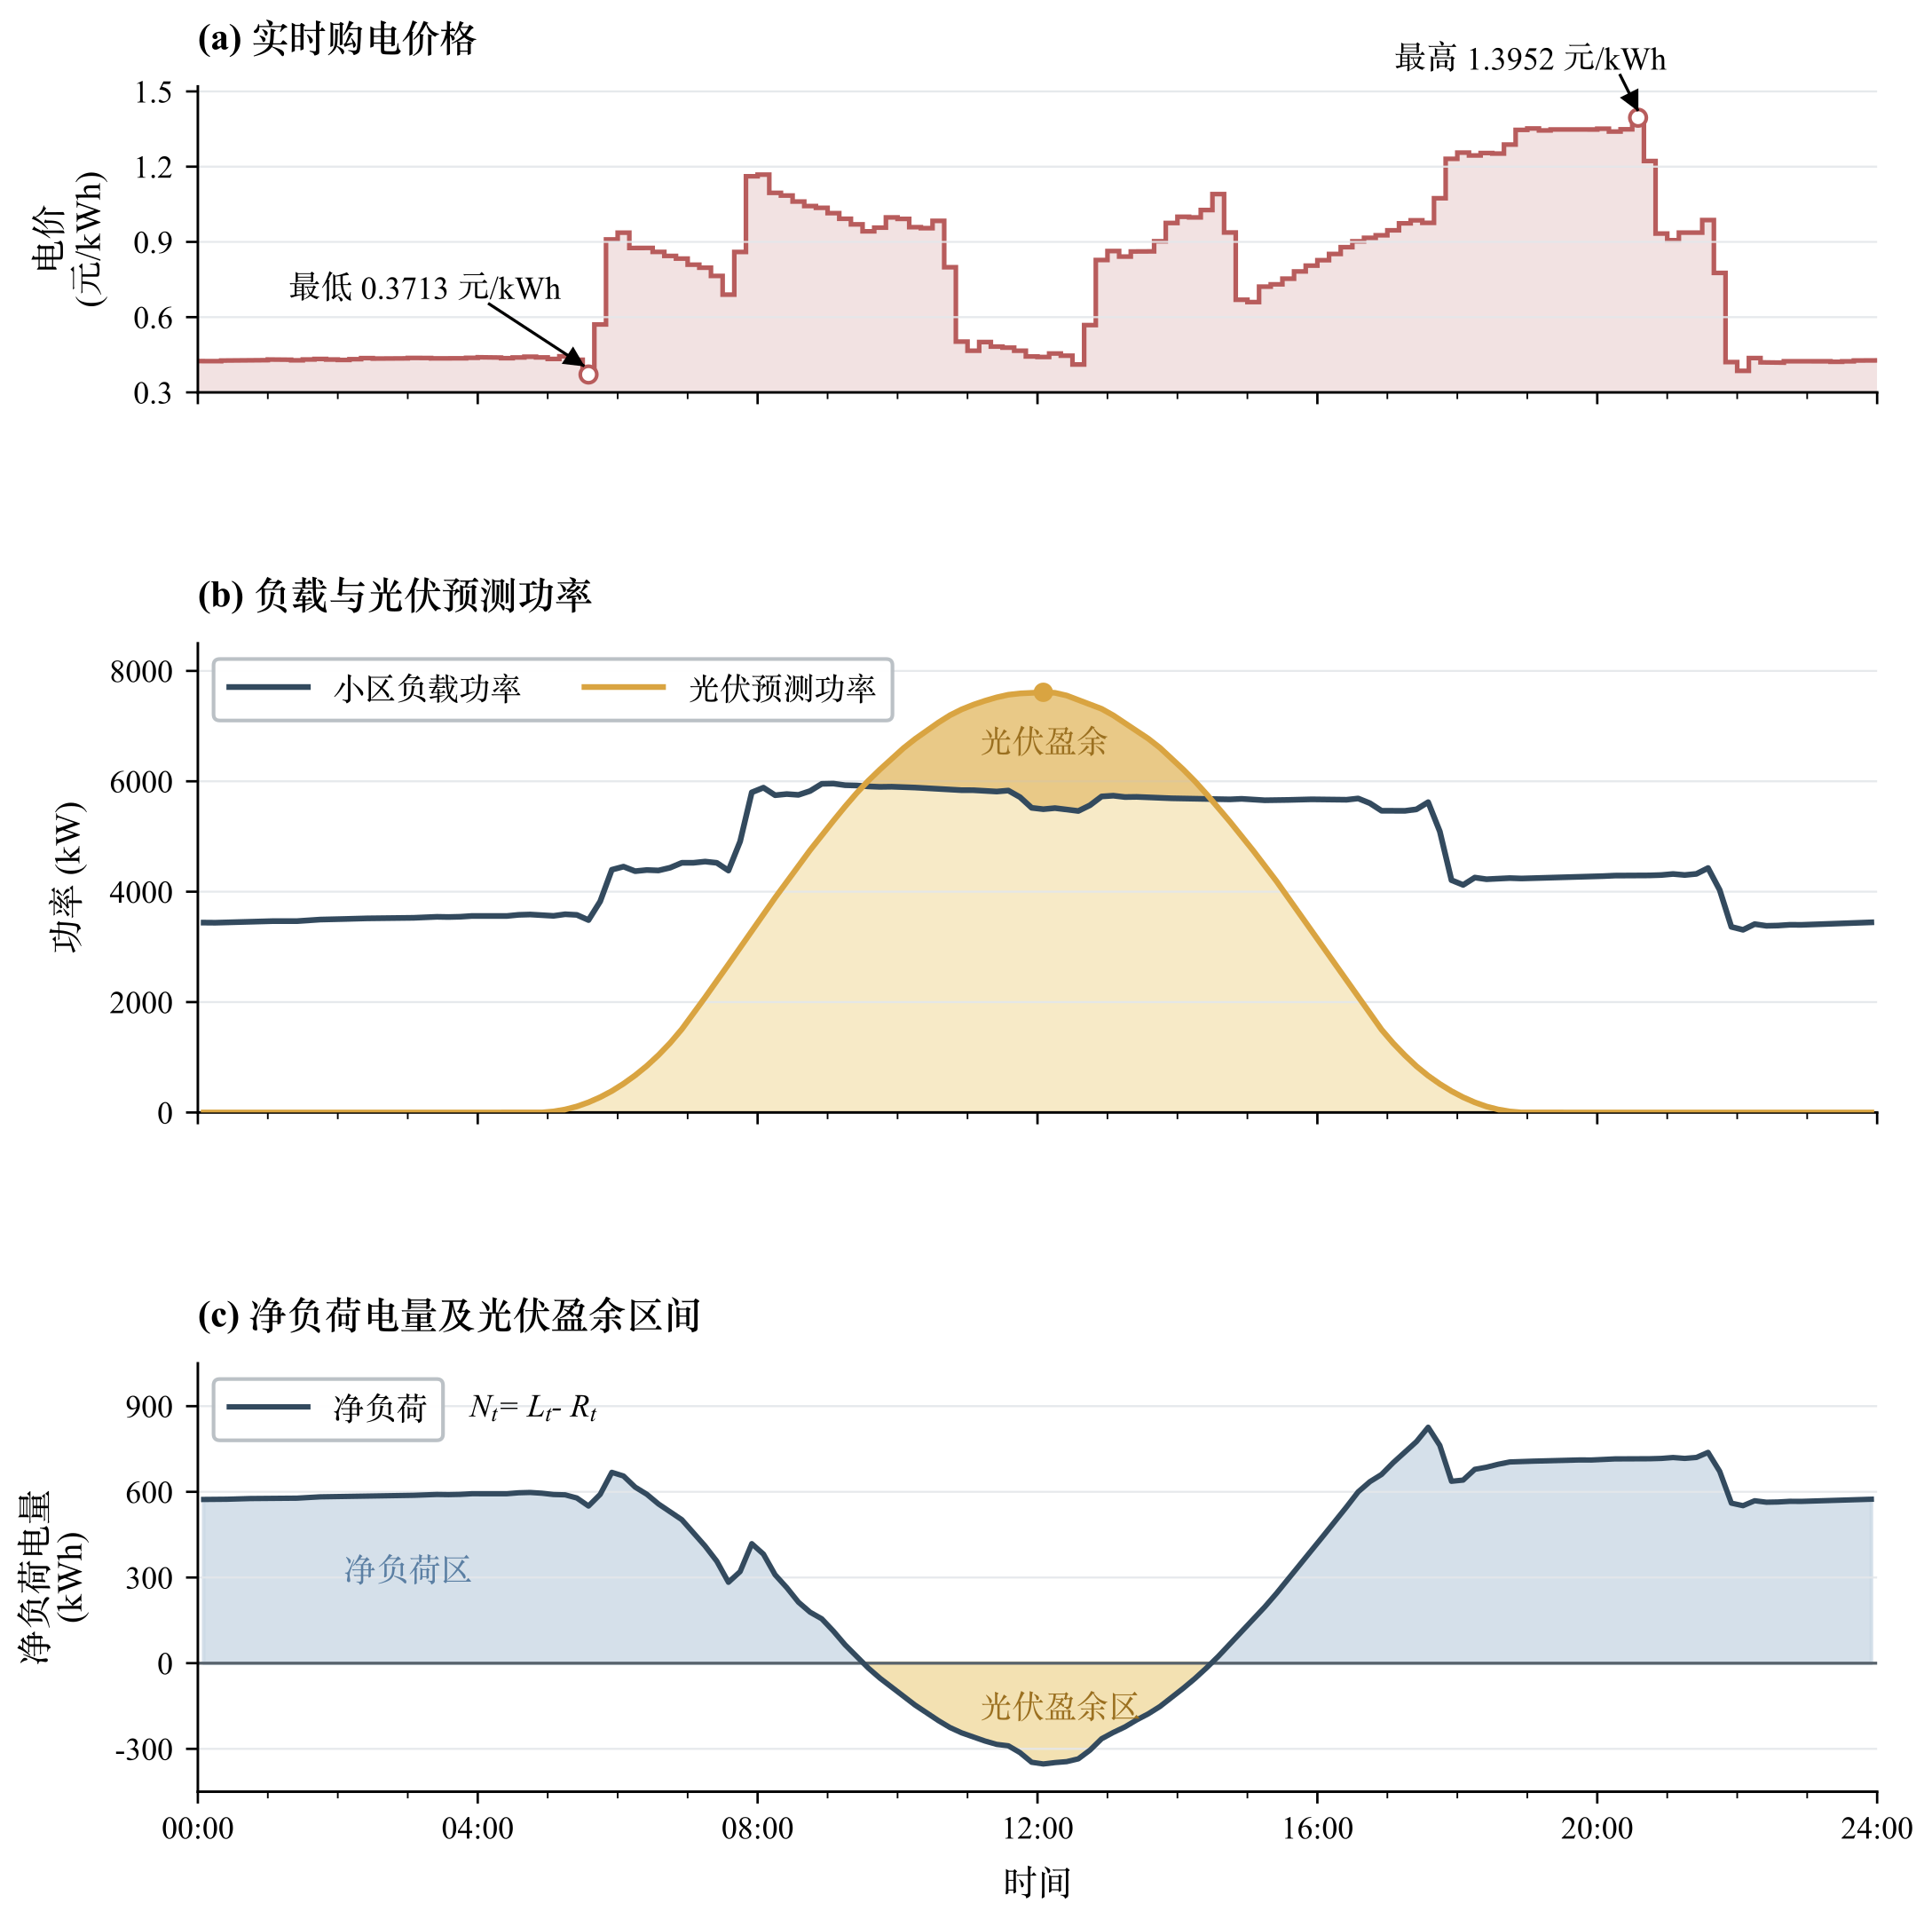
\includegraphics[width=0.55\textwidth]{figures/eda_01_daily_conditions.png}
  \caption{典型日电价、负载与光伏及净负荷特征}
  \label{fig:eda-daily-conditions}
\end{figure}

观察图~\ref{fig:eda-daily-conditions}，我们发现午间光伏不仅能够覆盖负载，还形成了一段净负荷为负的富余区间；傍晚光伏逐渐退出后，微网又需要较多外部供电。与此同时，凌晨和深夜电价较低，晚间电价较高。这说明微网面临的并非单纯的电量不足，而是发电、用电和购电价格在时间上的不匹配：午间有电可用，却未必能在当时全部消纳；晚间需要供电，又可能恰逢较高电价。

由此，储能的作用可以从两个角度理解。一是将午间富余光伏留待后续使用，提高清洁能源的本地消纳水平；二是利用低价时段充电，在高价时段减少外网购电，为改善经济性创造空间。两种作用不一定对应同一充放电安排，因此调度时不能只追随负载，也不能只追随电价，而应联合考虑全天供需与储能状态。

进一步比较后，我们还发现附件1的负载和光伏曲线与附件2的全年同刻均值几乎重合，说明典型日能够反映平均意义下的供需形状。不过，平均曲线也可能掩盖实际日期之间的差异，这促使我们继续考察全年数据。

\subsubsection{供需关系的月度变化}

查阅有关居民用电的资料可知，气温变化会通过制冷、采暖等需求影响用电；光伏出力则受日照和天气条件影响。\textsuperscript{\href{https://www.eia.gov/todayinenergy/detail.php?id=10211}{[2]}} \textsuperscript{\href{https://www.energy.gov/cmei/systems/solar-integration-solar-energy-and-storage-basics}{[1]}} 考虑到两者对季节变化的响应未必同步，我们对附件2按月汇总：先计算每日累计电量，再求各月的日均值，以避免月份天数不同带来的影响；同时选取3、6、9、12月，比较各月的平均日内净负荷，结果如图~\ref{fig:eda-monthly-netload}所示。

\begin{figure}[!htbp]
  \centering
  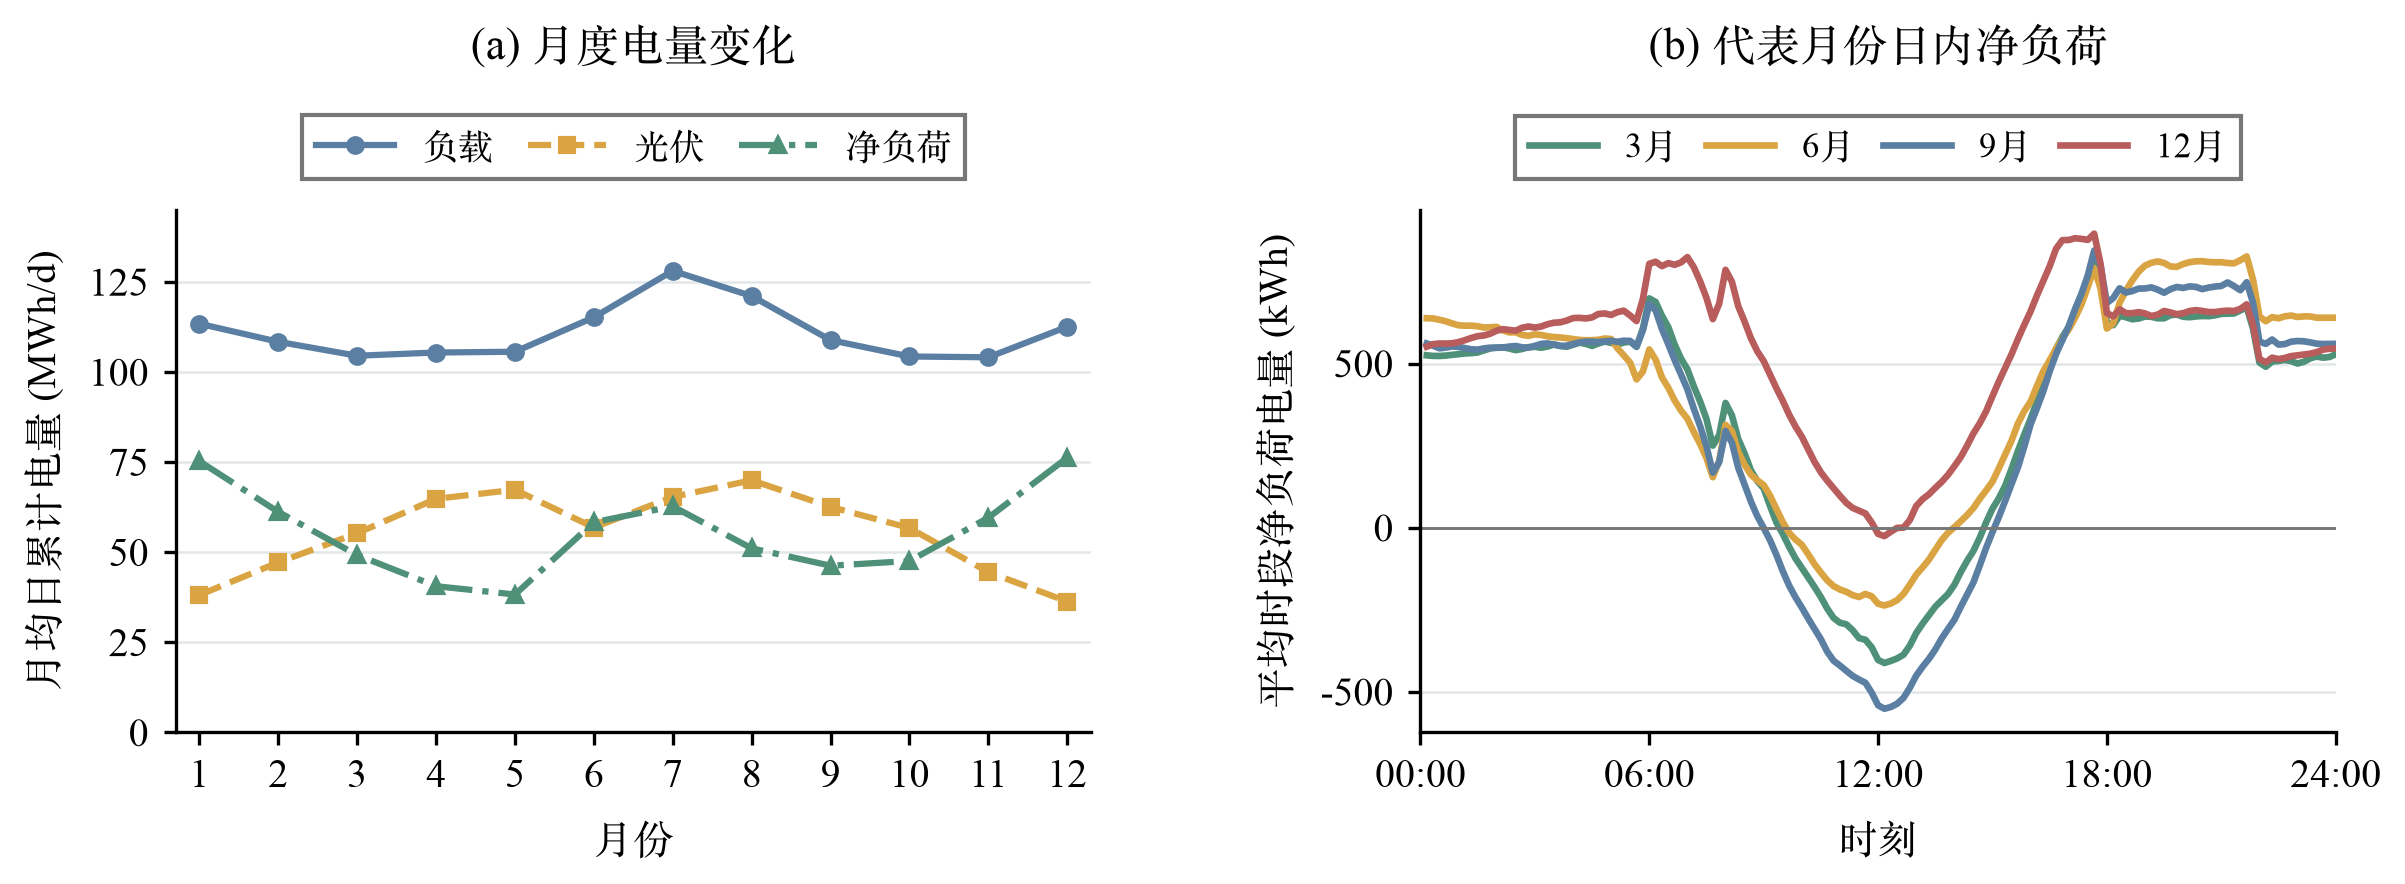
\includegraphics[width=0.95\textwidth]{figures/eda_02_monthly_netload.png}
  \caption{月均日累计电量与代表月份的平均时段净负荷}
  \label{fig:eda-monthly-netload}
\end{figure}

从图~\ref{fig:eda-monthly-netload}可以看出，负载与光伏并不是同步升降的。夏季负载虽有所增加，较充裕的光伏也能抵消部分供电需求；冬季光伏贡献减弱，净负荷则明显高于春末。这与居民用能和太阳能资源可能随季节变化的一般认识相符，意味着微网对外部供电的依赖取决于发电与用电的共同变化，不能仅根据负载大小判断。

我们进一步发现，不同月份的净负荷并非只存在总量差异，午间低谷的深度也明显不同：部分月份能够形成较充裕的光伏富余，冬季午间则接近供需平衡。这意味着，一套适合光伏充裕月份的储能安排，未必适合光伏不足的月份；后续决策既要关注当天需要多少电，也要关注这些电量在什么时刻出现。因此，历史样本的选择应考虑月份和季节相近性，而不宜将全年日期不加区分地混合使用。这里识别的是一年样本中的月度特征，尚不能据此确认稳定的年度周期。

\subsubsection{居民负载的周周期}

除天气因素外，考虑到工作日与休息日的交替可能改变居民在家时间和用电安排，负载还可能存在周尺度上的重复性。为检验这一点，我们比较相隔1--14天的同刻负载。由于每天共有的昼夜形状也会使相关性偏高，先减去各时段的全年平均负载，再计算日滞后相关系数，绘得图~\ref{fig:eda-weekly-lag}。

\begin{figure}[!htbp]
  \centering
  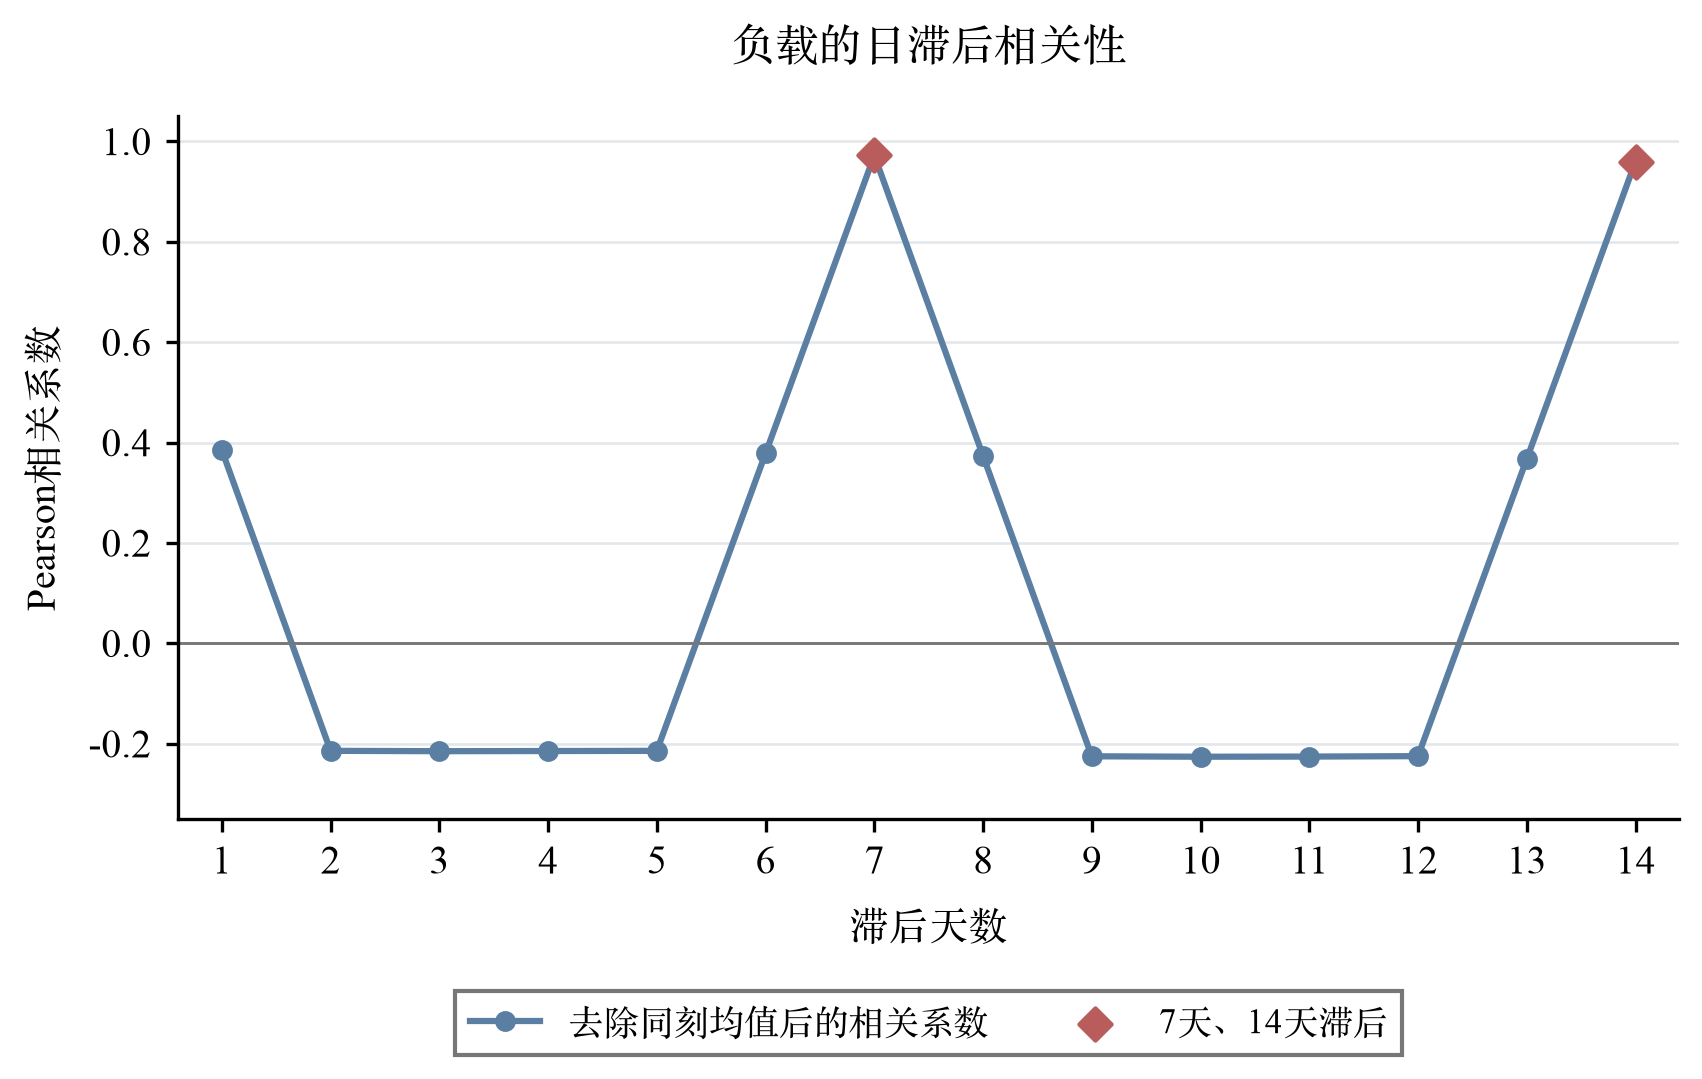
\includegraphics[width=0.64\textwidth]{figures/eda_03_weekly_lag.png}
  \caption{去除同刻均值后的负载日滞后相关性}
  \label{fig:eda-weekly-lag}
\end{figure}

我们发现，相关性在相隔7天和14天处形成明显峰值，且高于邻近滞后，说明负载在日际变化之外保留了较强的周周期。这与以周为单位的工作和生活节奏相吻合，也提示我们：距离最近的历史日期未必最有参考价值，上周同刻的数据反而可能更接近当天的用电模式。

\subsubsection{光伏预报不确定性与电价时变性}

此前的分析揭示了供需变化中的规律，但购电计划面向未来，预报能否准确反映未来的光伏出力，仍需进一步考察。另一方面，即使供需相近，价格变化也可能改变储能的经济价值。因此，我们将附件3预报与附件2同一目标整点的实际光伏功率对齐，在有实际观测的样本中计算不同提前时间的平均绝对误差（MAE）；同时将附件4按日期与日内时刻排列，直接绘出原始电价热力图，合并展示于图~\ref{fig:eda-forecast-price}。

\begin{figure}[!htbp]
  \centering
  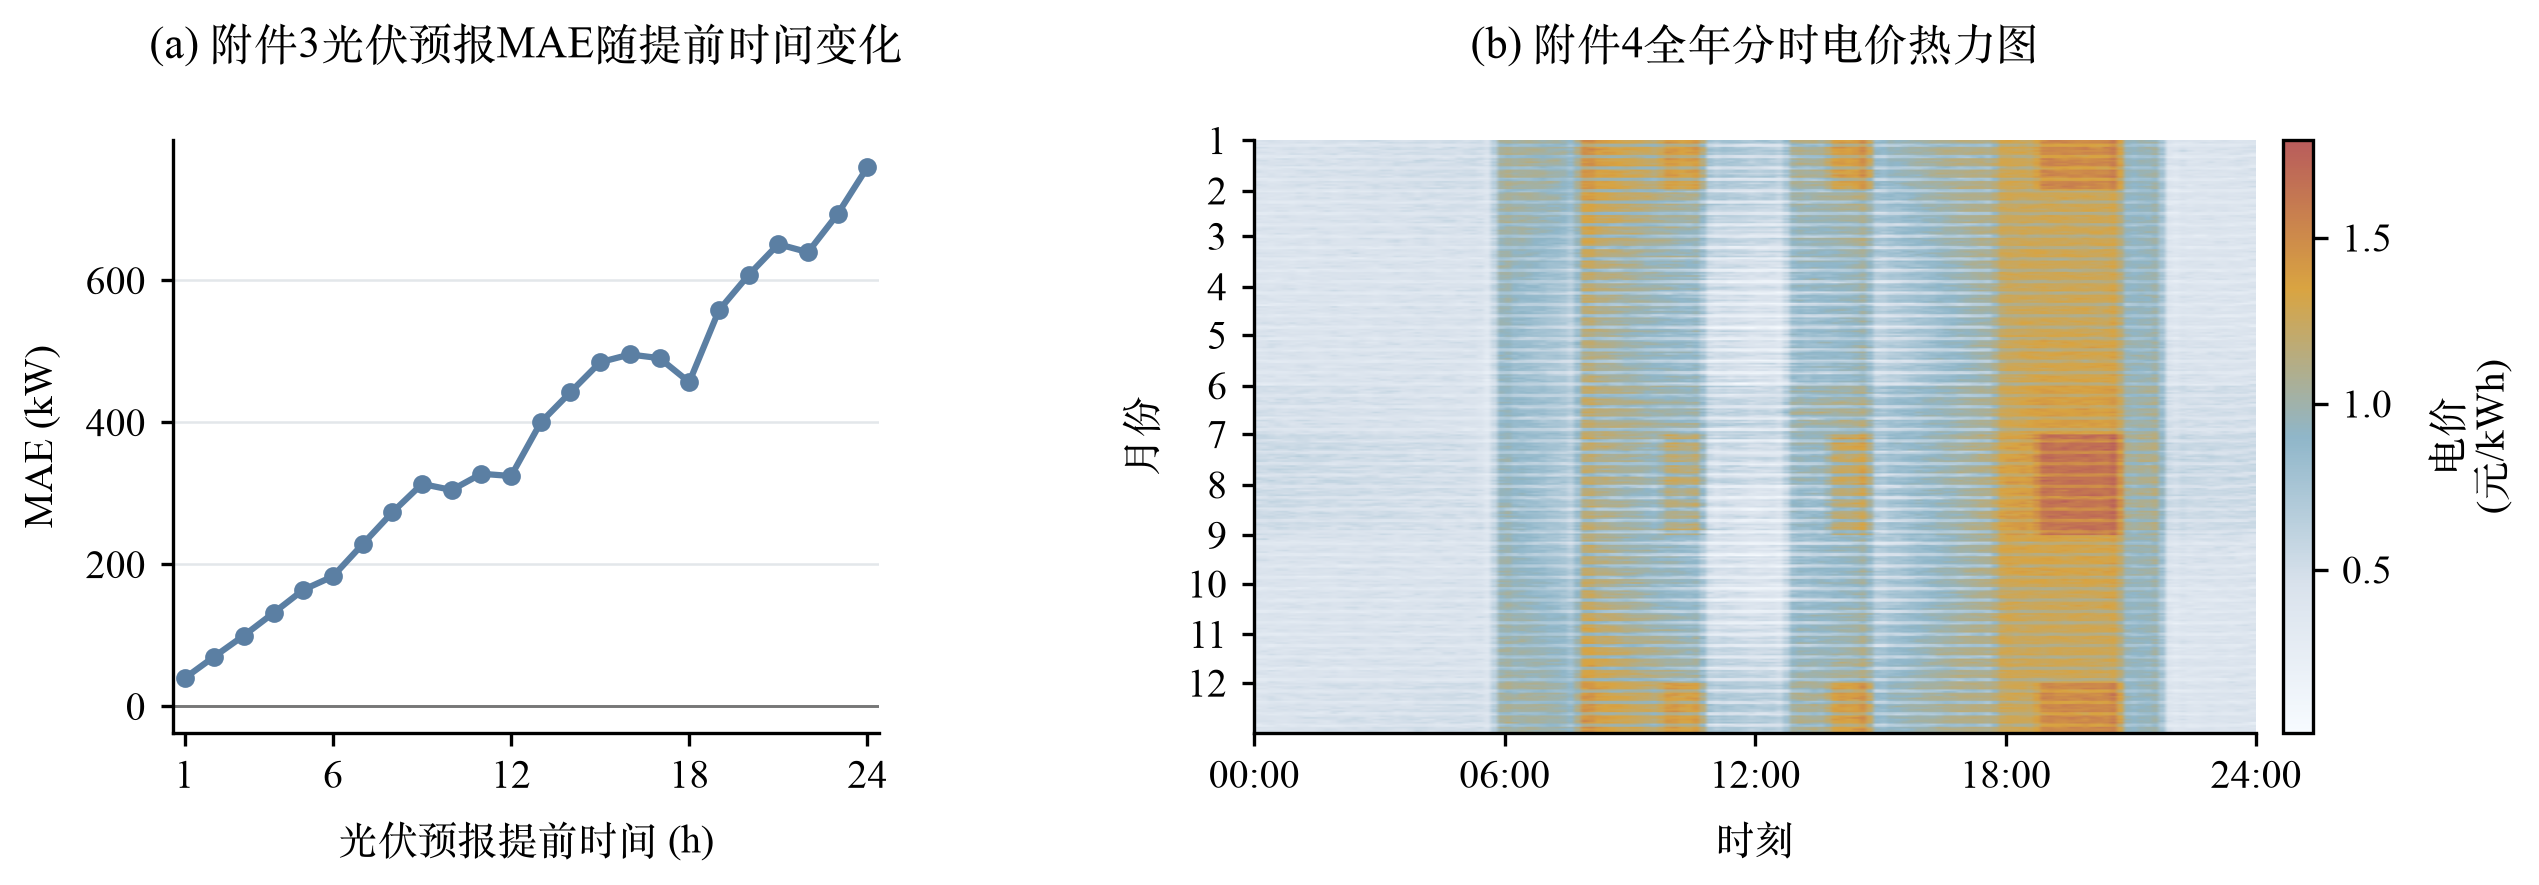
\includegraphics[width=0.95\textwidth]{figures/eda_04_forecast_price.png}
  \caption{光伏预报误差随提前时间变化与全年分时电价热力图}
  \label{fig:eda-forecast-price}
\end{figure}

观察图~\ref{fig:eda-forecast-price}(a)，我们发现预报误差随提前时间总体增大，近时刻预报较准确，远时刻偏差则更明显。这与已有研究中较长预测时距通常伴随较低预测精度的结论一致。\textsuperscript{\href{https://arxiv.org/abs/2111.02092}{[3]}} 为避免夜间大量近零值掩盖发电时段的偏差，图中仅统计预报值或实际值超过50~kW的样本。

从决策角度看，这说明日前预报不宜被当作确定的发电量。随着时间推进，更新预报可能为修正供需判断提供更有价值的信息，微网也有必要在初始计划之外保留调整空间。不过，预报更准确不等于调整一定更划算：减少紧急购电的收益还需与调整费用权衡，这正是后续研究滚动购电策略的关键。

图~\ref{fig:eda-forecast-price}(b)则表明，价格波动中仍保留了较清晰的日内峰谷结构，但同一时段的价格水平又随日期变化。这与电价通常受用电需求和发电成本等因素共同影响的背景相符。\textsuperscript{\href{https://www.eia.gov/energyexplained/electricity/prices-and-factors-affecting-prices.php}{[4]}} 我们据此认为，波动电价并未消除低价充电、高价放电的机会，却使固定时刻、固定电量的调度方式缺乏足够适应性。储能的价值不仅取决于能转移多少电量，还取决于何时转移、对应价差是否足以覆盖充放电损耗。

综合上述分析，我们发现光伏发电与居民用电在时间上存在错位，供需关系又随月份和生活节奏变化，预报偏差与电价波动进一步增加了调度的复杂性。这说明，微网的运行效益不仅取决于能够获得多少电能，更取决于能否在合适的时刻合理配置和利用电能。因此，研究光伏消纳、储能充放电与外网购电的协同优化，对于协调分布式发电与用电需求、保障小区供电并降低购电成本具有实际意义，也体现了微网在清洁能源本地利用与经济运行之间寻求平衡的必要性。上述分析也为后续刻画供需变化、预报不确定性与电价影响，建立购电与储能联合优化模型提供了数据依据。
